\chapter{Introduction}\label{chap:introduction}

Content Delivery Networks (CDNs) are responsible for the largest share of traffic in the Internet \cite{cisco2016}.
CDNs distribute popular content to caches in many geographical areas to save bandwidth by avoiding unnecessary multihop retransmission \cite{paschos2016wireless}.
By bringing the content geographically closer to the user, CDNs also reduce the latency of the services.
%TODO The exploitation of web caching and the invention of CDNs resolved the challenge of networks congestion.
%The growing

Four main stakeholders are interested in an efficient operation of CDNs.
End users expect high quality content and fast and reliable access.
The end users are direct customers of content providers, which have similar objectives.
To offer a good service to end users, content providers aim to provide high availability of their content, which is achieved by replicating content to many geographical areas.
At the same time they try to limit their expenditures for content servers and bandwidth offered by content delivery network providers.
In order to ensure an efficient replication of the content, content delivery network providers have a network of (globally) distributed interconnected datacenters at different points of presence.
The aim of content delivery network providers is to replicate the content to the areas of interest, while limiting their capital and operational expenditures for network and storage infrastructure.
The content provider and the content delivery network provider may be part of the same company.
Finally, Internet Service Providers (ISPs) are responsible for providing Internet access and for delivering the content to the end users.
ISPs aim to provide reliable and high speed Internet access, but try to keep the load on the network low and to reduce cost for connectivity with other ISPs.

%However, in today's Internet the inter-ISP traffic routing is based on a complex topology defined by inter-ISP relationships, e.g., peering or customer-to-provider, and ISP classifications such as \tier, large and small ISPs, and stub ISPs. Hence, these economic relations play an important role in the actual Internet traffic flow. However, this topology of the Internet is not taken into account by most evaluations of P2P guidance approaches, which limits the practical relevance of the results. Furthermore, it is an open question how much BitTorrent traffic is located in which region of the Internet. However, this is a prerequisite in order to estimate the potential of ALTO mechanisms.
%Therefore in this thesis, we model

In today's Internet new challenges arise in mobile networks.
The increasing number of mobile devices such as smart phones and tablets, high definition video content and high resolution displays result in a continuous growth in mobile traffic.
This growth in mobile traffic is further accelerated by newly emerging services, such as mobile live streaming and broadcasting services.
The steep increase in mobile traffic is expected to reach by 2018 roughly 60\% of total network traffic \cite{cisco2016}, the majority of which will be video.
%The next generation of 5G mobile networks prepares for 1000 times data challenge.
To handle the growth in mobile networks, the next generation of 5G mobile networks are designed to have higher access rates and an increased densification of the network infrastructure.

With the explosion of access rates and number of base stations the backhaul of wireless networks will become congested \cite{paschos2016wireless}.
To reduce the load on the backhaul the research community suggests to install caches in gateway routers between the wireless network and the Internet, in base stations of different sizes (small or regular size cells), and in end-user devices.
A recent approach \cite{valancius2009greening} proposes to augment spare capacities on customer premise equipment (CPE) such as home gateways or nano data-centers (NaDas) to assist content delivery, showing that there is a high potential to save energy, although the capacity of home gateways is small and the uplink is limited.
The content is transported in a peer-to-peer manner keeping the traffic within the autonomous system (AS).
The caches are organized in a hierarchy, where caches in the lowest tier are requested first and the request is forwarded to the next tier, if the requested object is not found.
Another example for a hierarchical caching system with bandwidth constraints are femto caching architectures \cite{golrezaei2013femtocaching}, where content is cached on femto-basestations with small capacity but with considerable storage space.
The potential of these approaches highly depends on the number of caches available and their capacity for content delivery.
%Our goal is to assess the potential of content delivery networks using a high number of caches with limited capacity.

The performance of hierarchical cache networks can be accurately determined by analytic models developed in recent work \cite{che2002hierarchical, martina2014unified}.
The models do not consider constraints that limit the capability of caches to upload content such as the bandwidth of the uplink.
%In the NaDa approach the upload bandwidth of caches is limited.
To account for a limited upload bandwidth of caches, in this thesis the hierarchical caching system is modeled as loss network consisting of a server for each of the caches.

To further increase the overall backhaul capacity, current concepts also consider multiple connections to the Internet, thereby sharing and aggregating available backhaul access link capacities.
%The question is which sharing policy to apply for which system characteristics.
Current approaches considers access link sharing among neighboring users based on offloading thresholds.
Each user should only share its access link for bandwidth offloading when having spare capacity, in order to avoid negatively affecting the own Internet connections.
%Therefore, two thresholds were introduced, i) a support threshold until which utilization a user will offer bandwidth to other users, and ii) an offloading threshold indicating from which utilization a user can offload to supporting neighbors.
It is hard and non-intuitive to determine the threshold settings for fair and effective operation of a bandwidth sharing system.
Therefore in this thesis a partial bandwidth sharing environment with offloading policy is investigated using an analytic model.
A direct application of the model is the aggregation of backhaul bandwidth by connecting neighboring access links.

The objectives of this monograph can be summarized as follows.
The first goal is to provide a thorough understanding of the nature of today's content delivery networks and their distribution of resources on AS level.
This knowledge allows to assess the costs produced by current content delivery approaches and to estimate their optimization potential.
Furthermore, we use this knowledge to design traffic management mechanisms that reduce costly inter-domain traffic and use spare resources in the backhaul to improve the overall system performance.
The second goal is to analyze the performance of hierarchical cache networks with limited capacity in order to assess their potential to support content delivery.
The final objective is to evaluate the performance of backhaul bandwidth aggregation systems.% in heterogeneous load conditions.

A detailed description of the scientific contribution in this monograph is given in the following.

%\section{Scope of Considered Stakeholders}\label{sec:introduction:considered_stakeholders}
\newpage
\section{Scientific Contribution}\label{sec:introduction:scientific_contribution}

This section summarizes the contribution of this monograph to the fields of hierarchical content delivery networks and the analysis of bandwidth aggregation systems.
An overview of the content of the studies is given and their relations are explained.

\begin{figure}
\centering
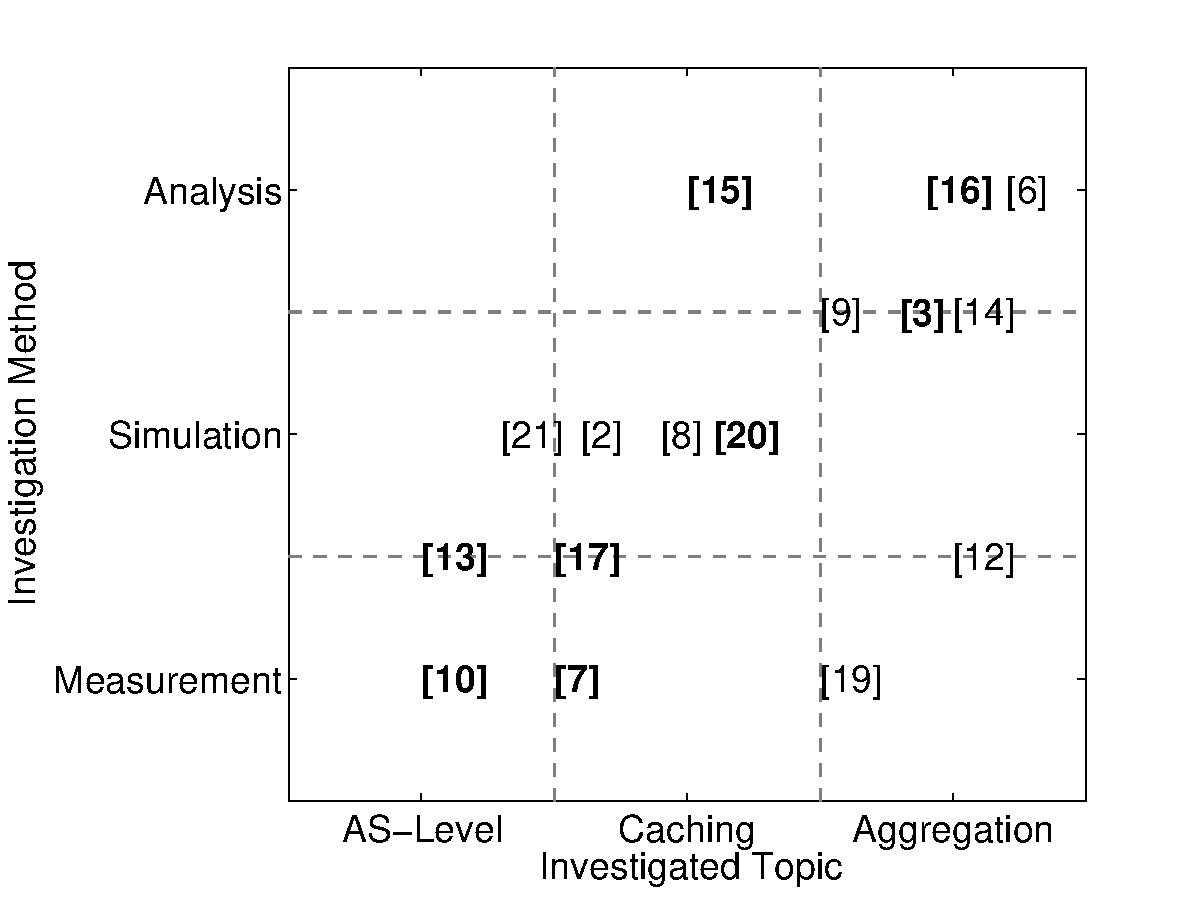
\includegraphics{figures/publications}
\caption{Cartography of scientific contributions of the author on performance evaluation of hierarchical content delivery networks. The content of references presented in this monograph is depicted in bold.}\label{fig:introduction:publications}
\end{figure}

\reffig{fig:introduction:publications} classifies the publications according to the investigated topic on the x-axis and the investigation methodology on the y-axis.
The investigated topics are the characterization of content delivery networks on AS-Level, caching systems and bandwidth aggregation systems.
The methods comprise real-world Internet measurements, simulations and analysis.
The studies may overlap different areas in both dimensions or only cover a single aspect and method, which means that a single subject is investigated using different methods or may comprise AS aware and caching mechanisms at the same time.

%In the theoretical area methods from queueing theory, mean value analysis and the analysis of random variables are used.
%Measurements were performed using testbeds and custom software tools.
%Simulation studies, performed using \gls{DES}, and created analysis tools are summarized in the practical area.

%Annotations are used to highlight scientific publications whose content contributes to the respective chapters.

The first major contribution of this monograph is a characterization of content delivery networks on AS level.
In order to characterize the server infrastructure of CDNs, a distributed measurement architecture is necessary, due to the location based server assignment in CDNs.
Typically distributed measurement platforms, which are generally not located in ISP networks, are used for that purpose.
% The problem is that these measurement platforms may not reflect the perspective as consumer, since they are hosted in National Research and Education Networks (NRENs) and not in ISP networks.
% We compare the capabilities of a crowdsourcing platform and a PlanetLab testbed for distributed active measurements.
To achieve a better view on the YouTube CDN from the perspective of end users in access networks we use a commercial crowdsourcing platform to recruit regular Internet users as measurement probes, c.f. \cite{burger2014vantage}.
Thus, we increase the coverage of vantage points for the distributed measurement of the YouTube CDN.
To evaluate the impact of the measurement platform and the coverage of their vantage points, we perform the same measurements using PlanetLab nodes and crowdsourcing users and compare the obtained results.
The results show that distributed measurements in PlanetLab are not capable to capture a globally distributed network, since the PlanetLab nodes are
located in National Research and Education Networks (NRENs) where the view on the Internet is limited.
The models derived from the measurement results can be used for performance analysis and optimization of content delivery mechanisms.
In particular the models are used to assess the overall potential of approaches using home routers to support content delivery.
In order to determine the amount of home routers available to support content delivery in ASs, we evaluate the Internet Census Dataset, which contains a complete scan of the IP address space, c.f. \cite{burger2016hierarchical}.
The evaluation shows that autonomous system size is highly heterogeneous, where the 10 largest autonomous systems already contain 30\% of the active IP addresses.
To model the traffic flow of P2P networks across ISPs in the Internet, we use measurements of live P2P networks and the actual AS topology of the Internet provided by Caida.org.
Thus, we estimate P2P traffic characteristics and the emerging transit costs.
Measurements of live P2P networks contain the location of peers in the Internet.
%The dataset from Caida.org contains a full AS graph derived from RouteViews BGP table snapshots, including the AS relations.
We use inferred AS paths to calculate the real AS paths between peers in the P2P networks and define three peer selection strategies that decide which peer is connected to which other peer, c.f. \cite{burger2012profit}.
Analysis of the optimization potential of P2P networks shows that the transit traffic is reduced especially in large ISPs by locality aware peer selection.
By estimating the potential of ISPs to optimize their revenue, we find that especially for small ISPs the potential to reduce transit costs is high using local peer selection.
%TODO results heterogeneous?
%They also serve as input for the optimization strategies for peer selection and the performance evaluation of hierarchical CDNs in realistic parameter studies.

%We develop a method to accurately assess the system performance of tiered caching architectures with bandwidth constraints.
As second major contribution, we evaluate the performance of a tiered caching architecture with bandwidth constraints analytically and by means of simulation.
We provide a versatile simulation framework for evaluating hierarchical caching systems allowing to consider different features including the home router sharing probability, bandwidth constraints and the AS topology.
We use the inferred AS paths to calculate the real AS paths and assess the transit cost savings by hierarchical caching systems, c.f. \cite{lareida2015augmenting,rbhorst-demo}.
We develop a method to accurately assess the system performance of tiered caching architectures with bandwidth constraints analytically.
%The models do not consider constraints that limit the capability of caches to upload content such as the bandwidth of the uplink.
%In the NaDa approach the upload bandwidth of caches is limited.
To consider the upload bandwidth the system is modeled as loss network consisting of a server for each of the caches.
The exact stationary distribution of the loss network is too complex to evaluate.
%In \cite{tan2013optimal} the system is analyzed under large system asymptotic where simplifications occur.
%We use a different approach by approximating the arrival rate of requests at the caches.
Approximating the arrival rate of requests at the cache allows us to effectively assess the loss probability by using a simple form of the Erlang formula for a loss network, c.f. \cite{burger2016hierarchical}.
Even for traffic with highly heterogeneous request rates the approximation reflects the system performance.
By comparing uncoordinated caching strategies using an overlay with optimal content placements in parameter studies, we find that the overall system performance can be further increased by more than 10\% if an optimal content placement is used.
The potential to increase the efficiency of the CDN is especially high if only a small or no ISP cache is available.
%TODO REPHRASE: During off-peak operation of the network, the users can cheaply populate their caches with parts of popular contents.

The third major contribution presented in this monograph considers the aggregation of backhaul bandwidth to further increase the overall system capacity by using spare bandwidth resources.
In a first step a two dimensional Markov model is developed to seamlessly evaluate the performance of systems between partitioning and complete sharing dependent on the threshold settings, c.f. \cite{burger2016phycom}.
The results show that, in contrary to the prevailing opinion, a complete sharing system can perform worse than a partitioned system if the load on the links is highly heterogeneous.
In order to extend the model to the case of more than two links an approximation of the state probabilities using a fixed point iteration is used, c.f. \cite{burger2017im}.
This is highly relevant for praxis, since in densely populated areas far more than two access links are available for aggregation.
Bandwidth sharing systems are designed to increase the throughput of systems that are currently overloaded by using spare bandwidth of under-utilized links.
In such situations the load on the links is highly heterogeneous.
By considering an outer and an inner composite system we are able to apply the method to the case of heterogeneous load, which is crucial to assess the full potential of the approach.
Our results show that an overloaded system can highly benefit, by receiving multiples of its own capacity, from spare bandwidth of underutilized cooperating systems.
Finally, we evaluate the robustness of the mechanism against free riders by prioritizing links and find that altruistic users may only lose slightly more bandwidth than in normal operation.
This is important, since a bandwidth sharing system that is running an inefficient offloading policy may be exploited by free riders that claim spare bandwidth by offloading traffic, but do not share any of their own bandwidth.

%Beyond this monograph,

\section{Outline of Thesis}\label{sec:introduction:outline}

The remainder of this monograph is structured as follows.
\refchap{chap:aslevel} shows the principles and recent developments of content delivery networks and characterize their resources on AS level by performing and evaluating distributed measurements.
In order to characterize P2P networks on AS level, we analyze a measurement study and identify the number of peers per swarm available in each AS and investigate the performance of different peer selection strategies.
We compare the capabilities of a crowdsourcing platform and a PlanetLab testbed for distributed active measurements.
To get a global view on the number of resources available in each AS we evaluate the Internet Census Dataset, which contains a complete scan of the IP address range.
The models derived are used to characterize the traffic in P2P networks and to develop optimization strategies to reduce inter-domain traffic and transit costs.

In \refchap{chap:hierarchical} we analyze hierarchical caching systems.
To this end, we introduce models for hierarchical caching systems, content popularity and traffic models and give an overview on existing analytical models.
We describe the simulation framework developed to evaluate hierarchical caching systems and give numerical examples studying the impact of caches on transit traffic.
Finally, we provide an analytic model for hierarchical caching systems considering bandwidth constraints of the caches and show the impact of limited bandwidth on the overall system performance.

In \refchap{chap:aggregation} we analyze the performance of bandwidth aggregation systems.
We first give an overview on bandwidth aggregation approaches and study existing performance models for bandwidth aggregation systems.
We define the system model and give analytic results of reference systems.
We then provide analytical models for bandwidth aggregation systems with two links and multiple links and show their potential in numerical examples.
We extend the analytical models to support imbalanced load in order to determine the full potential of bandwidth aggregation systems, which is achieved when spare bandwidth can be reused.
Finally, we study the fairness of the system and provide results with general service times.
\refchap{chap:conclusion} summarizes this monograph and draws conclusions.
